\documentclass[letter, 10pt]{article}
\usepackage[utf8]{inputenc}
\usepackage[T1]{fontenc}
\usepackage[spanish]{babel}
\usepackage{amsfonts}
\usepackage{amsmath}
\usepackage{graphicx}
\usepackage{url}
\usepackage[top=3cm,bottom=3cm,left=3.5cm,right=3.5cm,footskip=1.5cm,headheight=1.5cm,headsep=.5cm,textheight=3cm]{geometry}
\usepackage{float}
\usepackage{tikz}
\usetikzlibrary{shapes.geometric, arrows.meta, positioning}

% Entorno de pseudocodigo (estilo "ruled"), sin paquetes externos de algoritmos
\floatstyle{ruled}
\newfloat{algorithm}{tbp}{loa}
\floatname{algorithm}{Algoritmo}



\begin{document}
\title{Inteligencia Artificial \\ \begin{Large}Entrega 2: Electric Vehicle Charging Station Placement Problem (EVCSPP)\end{Large}}
\author{Matias Lara Plaza}
\date{\today}
\maketitle


%--------------------No borrar esta secci\'on--------------------------------%
\section*{Evaluaci\'on}

\begin{tabular}{ll}
Mejoras 2da Entrega (10 \%): &  \underline{\hspace{2cm}}\\
C\'odigo Fuente (10 \%): &  \underline{\hspace{2cm}}\\
Representaci\'on (5 \%):  & \underline{\hspace{2cm}} \\
Descripci\'on del algoritmo (15 \%):  & \underline{\hspace{2cm}} \\
Experimentos (10 \%):  & \underline{\hspace{2cm}} \\
Resultados (40 \%):  & \underline{\hspace{2cm}} \\
Conclusiones (10 \%): &  \underline{\hspace{2cm}}\\
 &  \\
\textbf{Nota Final (100)}:   & \underline{\hspace{2cm}}
\end{tabular}
%---------------------------------------------------------------------------%
\vspace{2cm}


\begin{abstract}
El presente informe aborda el Problema de Ubicación de Estaciones de Carga para
Vehículos Eléctricos (EVCSPP), un problema de optimización combinatoria NP-duro que busca
determinar las ubicaciones óptimas para construir estaciones de carga en una red urbana,
minimizando el costo de construcción y garantizando criterios de accesibilidad, satisfacción de
demanda y cobertura territorial. Para resolverlo se implementó un algoritmo genético con
codificación binaria, manejo de las restricciones por penalización y un criterio de parada por
estancamiento. El algoritmo se evaluó sobre instancias reales de 100 ubicaciones mediante un
barrido de 250 corridas que combinó el coeficiente $\alpha$ del problema con el tamaño de la
población, empleando distintas semillas como réplicas. Los resultados muestran, por un lado, que el
aumento de $\alpha$ conduce a redes más dispersas y realistas hasta una frontera a partir de la
cual el problema se vuelve infactible por construcción; y, por otro, que en este problema el
esfuerzo computacional, y no el tamaño de la población, es la palanca del rendimiento: una
población pequeña alcanza soluciones de menor costo que una veinte veces mayor, gastando alrededor
de dieciséis veces menos evaluaciones de la función de aptitud.
\end{abstract}
\newpage

\section{Introducci\'on}
La dependencia global de los combustibles fósiles ha sido durante décadas uno de los
principales motores del desarrollo económico y social, pero también una de las fuentes 
más significativas de emisiones de gases de efecto invernadero. El sector del transporte 
es uno de los mayores contribuyentes a esta problemática, siendo responsable de una 
fracción considerable de las emisiones globales de dióxido de carbono. Frente a este 
escenario, la electrificación del transporte ha emergido como una de las respuestas más 
concretas y escalables para reducir la huella ambiental de la movilidad urbana.

En este contexto, diversas regiones del mundo han comenzado a implementar marcos 
regulatorios y políticas públicas orientadas a acelerar la adopción masiva de vehículos 
eléctricos. La Unión Europea, por ejemplo, ha establecido objetivos vinculantes para la 
reducción de emisiones del sector transporte, impulsando tanto la electrificación de la 
flota vehicular como el desarrollo de infraestructura de carga a escala continental. Estas 
iniciativas han generado un crecimiento sostenido en el número de vehículos eléctricos 
en circulación, lo que a su vez ha puesto en evidencia una necesidad crítica: la 
planificación estratégica de las estaciones de carga.

La ubicación de estas estaciones no es un problema trivial. Una red de carga mal 
distribuida puede generar zonas sin cobertura, saturar ciertas ubicaciones y dejar a los 
conductores expuestos a la llamada ansiedad de rango, es decir, el temor a quedarse sin 
energía antes de alcanzar un punto de recarga. Por el contrario, una red bien planificada 
puede extender el alcance efectivo de los vehículos eléctricos a toda el área urbana, 
reducir costos de infraestructura y fomentar la adopción del transporte eléctrico.

El presente informe aborda precisamente este desafío a través del Problema de Ubicación
de Estaciones de Carga para Vehículos Eléctricos (EVCSPP, por sus siglas en inglés).
Más allá de revisar el estado del arte, este trabajo formula el problema, implementa un
algoritmo genético para resolverlo y evalúa experimentalmente su comportamiento, con foco
en el efecto del coeficiente $\alpha$ del problema y en el ajuste del tamaño de la población.
El documento se organiza como sigue: la Sección 2 presenta la definición formal del problema y sus variantes; la Sección 3 desarrolla el estado del arte sobre las principales técnicas propuestas en la literatura para resolverlo; la Sección 4 expone el modelo matemático que formaliza el problema de optimización; la Sección 5 detalla la representación de las soluciones empleada; la Sección 6 describe el algoritmo implementado; la Sección 7 presenta la metodología y los experimentos realizados; la Sección 8 reporta y analiza los resultados obtenidos; y la Sección 9 sintetiza las conclusiones del trabajo y propone direcciones de investigación futura.

\section{Definici\'on del Problema}

El Problema de Ubicac\'ion de Estaciones de Carga para Veh\'iculos El\'ectricos (EVCSPP, por sus siglas en ingl\'es) surge en el contexto de la electrificaci\'on del transporte, un pilar fundamental para el desarrollo de ciudades inteligentes y la mitigaci\'on de las emisiones de gases de efecto invernadero. A diferencia de las estaciones de combustible tradicionales, la recarga de veh\'iculos el\'ectricos requiere tiempos m\'as prolongados y est\'a limitada por la autonom\'ia de las bater\'ias, lo que genera ansiedad en los conductores. En este escenario, el EVCSPP consiste en determinar las localizaciones geogr\'aficas estrat\'egicas para instalar infraestructuras de carga dentro de una red de transporte, garantizando que los usuarios puedan desplazarse por toda la \'area urbana sin agotar su energ\'ia.

\textbf{El objetivo principal de este problema de optimizaci\'on es minimizar los costos totales del sistema.} Esto abarca fundamentalmente el costo de construcci\'on e instalaci\'on de las estaciones (terrenos, equipos, mantenimiento) y, dependiendo del enfoque, el costo de acceso o transporte, que representa la distancia que los usuarios deben recorrer para llegar a un punto de carga. Este objetivo persigue un equilibrio econ\'omico sin sacrificar la conveniencia de los conductores ni la cobertura del servicio.


La principal dificultad del EVCSPP radica en su elevada complejidad computacional, estando clasificado formalmente como un problema NP-duro \cite{1_Solving_optimal_evcsp_problem_QUANTUM}\cite{2_EVCSP_2013-ieee-conference}.
A medida que aumenta el tama\~no de la red y el n\'umero de ubicaciones candidatas, el espacio de soluciones crece de manera exponencial. La intrincada interdependencia entre m\'ultiples dimensiones (como la infraestructura vial, las limitaciones el\'ectricas y el comportamiento del usuario) hace que los m\'etodos de optimizaci\'on exactos sean ineficientes a gran escala, requiriendo el uso de algoritmos heur\'isticos, metaheur\'isticos o computaci\'on de inspiraci\'on cu\'antica para encontrar soluciones viables.

En la formulaci\'on del problema interact\'uan diversas constantes y variables clave. Las constantes reflejan el entorno f\'isico y econ\'omico: los nodos o sitios candidatos en la ciudad, las distancias entre ellos, la autonom\'ia promedio de los veh\'iculos, la demanda de carga local estimada (basada en el flujo de tr\'afico o densidad poblacional), la capacidad m\'axima de suministro por estaci\'on y los costos fijos asociados a cada locaci\'on. Por su parte, las variables definen el comportamiento del modelo; la principal es una variable de decisi\'on de naturaleza binaria que simplemente indica si se construye o no una estaci\'on en un sitio espec\'ifico\cite{1_Solving_optimal_evcsp_problem_QUANTUM}.

Para que una soluci\'on sea v\'alida, debe cumplir con restricciones operativas y geom\'etricas estrictas. La primera es la restricci\'on de cobertura o alcance, la cual exige que la distancia entre cualquier par de estaciones contiguas no supere la capacidad de conducci\'on aut\'onoma del veh\'iculo, asegurando as\'i una red interconectada. La segunda es la satisfacci\'on de la demanda, que obliga a que la suma de las capacidades de las estaciones operativas en un radio determinado logre cubrir \'integramente las necesidades de carga de los residentes locales\cite{1_Solving_optimal_evcsp_problem_QUANTUM}. Adicionalmente, existen restricciones de asignaci\'on exclusiva que fuerzan a que cada sector de la ciudad est\'e vinculado a una instalaci\'on operativa, y restricciones de equidad territorial para asegurar que la cobertura abarque la totalidad de la zona urbana, incluyendo \'areas remotas o de menor tr\'ansito\cite{1_Solving_optimal_evcsp_problem_QUANTUM}.

Finalmente, a partir de esta estructura cl\'asica, han surgido diversas variantes del problema adaptadas a redes modernas. Destacan los problemas conjuntos de ubicaci\'on y dimensionamiento (sizing), que no solo deciden d\'onde construir sino cu\'anta potencia asignar a cada estaci\'on\cite{2_EVCSP_2013-ieee-conference}; el EVCSPP integrado con sistemas de Veh\'iculo a Red (V2G), donde el autom\'ovil no solo consume sino que provee energ\'ia a la red el\'ectrica\cite{2_EVCSP_2013-ieee-conference}; modelos de planificaci\'on de dos etapas que incorporan la incertidumbre de los Recursos Energ\'eticos Distribuidos (DER), como la energ\'ia solar o e\'olica\cite{3_optimal_placement-metaheuristic}; y las formulaciones basadas en el modelo p-mediano, centradas espec\'ificamente en minimizar la distancia ponderada de viaje de todos los usuarios hacia un n\'umero fijo y predeterminado de estaciones\cite{3_optimal_placement-metaheuristic}.


\section{Estado del Arte}


El estudio de la ubicación espacial de instalaciones tiene sus raíces teóricas a principios del siglo XX con el problema de la planta industrial introducido por Alfred Weber\cite{4_survey_FLP}. Sin embargo, el Problema de Ubicación de Estaciones de Carga para Vehículos Eléctricos (EVCSPP, por sus siglas en inglés) surge en un contexto contemporáneo y diferenciado, impulsado por la imperiosa necesidad de mitigar las emisiones de gases de efecto invernadero procedentes del sector transporte y de reducir la dependencia mundial de los combustibles fósiles\cite{7_recent_trends_optimization_techniques}. Este problema cobra especial relevancia estratégica con la transición hacia el desarrollo de ciudades inteligentes, donde la infraestructura de transporte no solo debe proveer una cobertura espacial sino que también debe integrarse de forma sinérgica y segura con la red eléctrica tradicional\cite{6_EVCSP_formulation_complexity}. El sostenido crecimiento del interés académico en esta área se aprecia tanto en el campo general de la ubicación de instalaciones (ver Figura~\ref{fig:publicaciones_anuales}) como, de manera más específica, en la optimización de infraestructura de carga para vehículos eléctricos (ver Figura~\ref{fig:publicaciones_rahman}).

\begin{figure}[h]
    \centering
    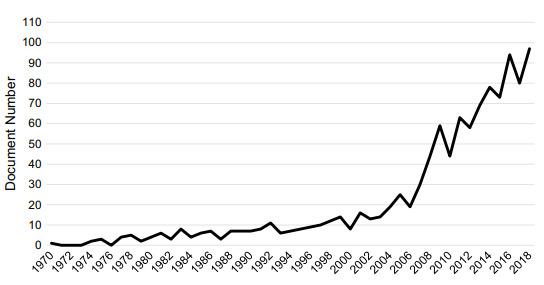
\includegraphics[width=0.7\textwidth]{images/fig1_Celik_Turkoglu.jpg}
    \caption{Evolución anual del número de publicaciones sobre 
    problemas de ubicación de instalaciones de servicio, evidenciando 
    el crecimiento sostenido del campo a partir del año 
    2000 \cite{4_survey_FLP}.}
    \label{fig:publicaciones_anuales}
\end{figure}

\begin{figure}[h]
    \centering
    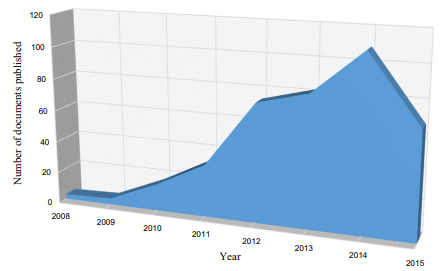
\includegraphics[width=0.7\textwidth]{images/rahman_fig2.png}
    \caption{Número de publicaciones anuales sobre optimización de 
    infraestructura de carga para vehículos eléctricos e híbridos 
    enchufables registradas en bases de datos científicas entre 2008 
    y 2015, reflejando el rápido crecimiento del área de 
    investigación \cite{7_recent_trends_optimization_techniques}.}
    \label{fig:publicaciones_rahman}
\end{figure}


Para abordar este problema, formalmente clasificado por la complejidad computacional como NP-duro, la comunidad científica ha empleado una evolución de enfoques que parten de modelos matemáticos estrictos hacia técnicas de inteligencia artificial. Inicialmente, se aplicaron métodos de optimización exacta, como la programación lineal entero-mixta (MILP) y algoritmos de branch-and-bound, los cuales buscan la optimalidad matemática calculando todas las interacciones posibles\cite{6_EVCSP_formulation_complexity}. No obstante, el crecimiento exponencial del espacio de búsqueda derivado del tamaño de las redes urbanas modernas hizo que estas técnicas resultaran ineficientes y colapsaran en la práctica. Como respuesta, la resolución ha migrado sostenidamente hacia el uso de algoritmos heurísticos y, de manera predominante, métodos metaheurísticos, que sacrifican la garantía absoluta del óptimo a cambio de aproximaciones de alta calidad en tiempos de cómputo razonables\cite{4_survey_FLP}\cite{5_Metaheuristic_FLP}.

En cuanto a las representaciones que han logrado modelar la complejidad del EVCSPP de forma más efectiva, destacan los algoritmos poblacionales y las rutinas basadas en memoria adaptativa. Históricamente, los Algoritmos Genéticos (GA) y la Búsqueda Tabú (TS) han sido las representaciones discretas dominantes para problemas de ubicación de instalaciones, demostrando gran flexibilidad en redes no capacitadas y modelos de p-mediano\cite{5_Metaheuristic_FLP}. Más recientemente, representaciones basadas en inteligencia de enjambres, como la Optimización por Enjambre de Partículas (PSO) y metaheurísticas inspiradas en la naturaleza, como la Optimización por Reacción Química (CRO), han demostrado ser excepcionalmente eficaces\cite{6_EVCSP_formulation_complexity}\cite{7_recent_trends_optimization_techniques}.La efectividad de estas representaciones radica en su intrínseca capacidad de resistencia frente a la escala del problema, permitiendo explorar vastas regiones del espacio de soluciones y evadir los óptimos locales mediante un equilibrio dinámico entre la diversificación (exploración) y la intensificación (explotación) de las alternativas\cite{6_EVCSP_formulation_complexity}\cite{7_recent_trends_optimization_techniques}.

Los resultados más destacados obtenidos hasta la fecha muestran una clara bifurcación operativa en función de la envergadura del escenario analizado. Para microrredes o instancias con un número reducido de nodos (generalmente por debajo de 150), los solucionadores exactos comerciales logran la optimalidad absoluta, aunque a expensas de un alto costo temporal\cite{6_EVCSP_formulation_complexity}. Por el contrario, en problemas a escala urbana, las técnicas metaheurísticas ostentan los resultados más sólidos: mientras que representaciones como GA han dominado consistentemente en tiempos de resolución computacional frente a otros métodos en problemas de cobertura máxima, algoritmos avanzados como CRO han probado superar ampliamente a los métodos constructivos o codiciosos (greedy), logrando convergencias ultra-rápidas hacia el óptimo global sin padecer los déficits de memoria que inutilizan a los modelos puramente matemáticos\cite{5_Metaheuristic_FLP}\cite{6_EVCSP_formulation_complexity}. Un caso ilustrativo de aplicación a escala real es la planificación de estaciones de carga en la ciudad de Hong Kong (ver Figura~\ref{fig:mapa_hk}), abordada mediante una combinación de métodos exactos y metaheurísticos\cite{6_EVCSP_formulation_complexity}.

\begin{figure}[h]
    \centering
    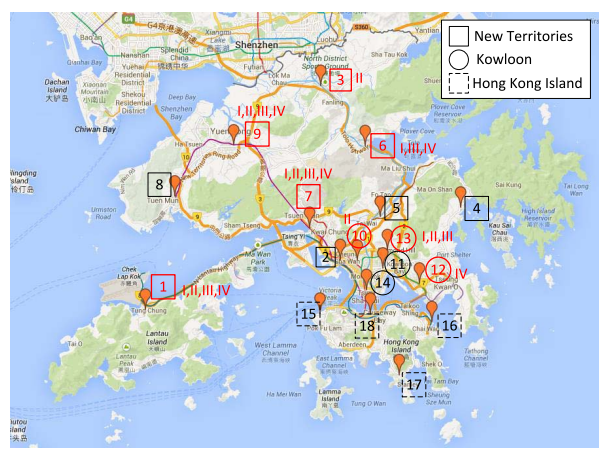
\includegraphics[width=0.6\textwidth]{images/lam_fig4.png}
    \caption{Distribución geográfica de ubicaciones seleccionadas para 
    la construcción de estaciones de carga en Hong Kong, correspondiente 
    a una aplicación real del EVCSPP resuelta mediante métodos exactos 
    y metaheurísticos \cite{6_EVCSP_formulation_complexity}.}
    \label{fig:mapa_hk}
\end{figure}

La tendencia actual de la investigación se está alejando progresivamente de la optimización simple y de las metaheurísticas puras para adentrarse en el desarrollo de técnicas híbridas y algoritmos de optimización multiobjetivo\cite{5_Metaheuristic_FLP}\cite{7_recent_trends_optimization_techniques}.
Las limitaciones de los métodos tempranos, que evaluaban únicamente el costo de instalación de las estaciones o la cobertura espacial del usuario, han propiciado el diseño de modelos complejos (como NSGA-II o MOPSO) que equilibran de manera simultánea factores en conflicto, como el costo de la red, el 'afeitado de picos' de la demanda eléctrica y el desgaste de las baterías\cite{7_recent_trends_optimization_techniques}. Hacia el futuro, el estado del arte se dirige invariablemente a integrar el despliegue físico de las estaciones con sistemas de Gestión de la Demanda (DSM), la implementación de arquitecturas de Vehículo a Red (V2G) y el acoplamiento directo de fuentes de energía renovable, particularmente la tecnología fotovoltaica, con el propósito de descentralizar la carga y proteger la integridad operativa de la red eléctrica principal\cite{7_recent_trends_optimization_techniques}.


\section{Modelo Matem\'atico}

El presente modelo matemático se basa en la formulación propuesta por Ou et al. (2025) \cite{1_Solving_optimal_evcsp_problem_QUANTUM}, 
quienes extienden el trabajo seminal de Lam et al. (2013) \cite{2_EVCSP_2013-ieee-conference} incorporando restricciones 
adicionales de cobertura urbana y zonas remotas. El problema consiste en determinar las 
ubicaciones óptimas para la construcción de estaciones de carga de vehículos eléctricos, 
minimizando el costo total de construcción y garantizando que la red resultante satisfaga 
criterios de accesibilidad, demanda y cobertura territorial.

\subsection{Conjuntos y Parámetros}

Se define un grafo no dirigido $G = (V, E)$, donde $V$ representa el conjunto de ubicaciones 
candidatas para la construcción de estaciones de carga y $E$ el conjunto de aristas que conectan 
dichas ubicaciones. A partir de un coeficiente de descuento $\alpha \in [0, 1)$ y el rango de 
autonomía promedio $R$, se define el subconjunto de nodos relevantes como:

\[
\bar{V} = \{j \in V \mid \alpha R \leq d(i,j) \leq R,\ i \neq j\}
\]

donde $d(i,j)$ denota la distancia entre los nodos $i$ y $j$. Este conjunto captura las 
ubicaciones que se encuentran suficientemente alejadas entre sí para evitar concentración 
excesiva de estaciones, pero dentro del rango de autonomía del vehículo.

Los parámetros del modelo se describen en el Cuadro~\ref{tab:parametros}.

\begin{table}[h]
\centering
\caption{Parámetros del modelo matemático}
\label{tab:parametros}
\begin{tabular}{cl}
\hline
\textbf{Parámetro} & \textbf{Descripción} \\
\hline
$C_j$       & Costo de construcción de la estación en la ubicación $j$, \\
            & incluyendo adquisición de terreno, construcción y operación \\
$R$         & Distancia de autonomía promedio de los vehículos eléctricos \\
$\alpha$    & Coeficiente de descuento que regula la densidad mínima entre estaciones \\
$d(i,j)$   & Distancia entre las ubicaciones $i$ y $j$ \\
$s_j$       & Radio de servicio de la estación en la ubicación $j$ \\
$D_j$       & Demanda de carga en la ubicación $j$ \\
$f_i$       & Capacidad de carga promedio en la ubicación $i$ \\
$\mathit{CityArea}$ & Área total de la ciudad que debe ser cubierta por las estaciones \\
$T$         & Subconjunto de ubicaciones candidatas en zonas remotas \\
\hline
\end{tabular}
\end{table}

\subsection{Variable de Decisión}

La variable de decisión del modelo es binaria e indica si se construye o no una estación 
de carga en cada ubicación candidata:

\[
x_j = \begin{cases} 1 & \text{si se construye una estación en la ubicación } j \\ 
0 & \text{en caso contrario} \end{cases} \quad \forall j \in V
\]

\subsection{Función Objetivo}

Se minimiza el costo total de construcción de las estaciones seleccionadas:

\[
\min \sum_{j=1}^{n} C_j x_j \quad \forall j \in V \tag{1}
\]

La función objetivo busca determinar el subconjunto de ubicaciones candidatas sobre las 
cuales construir estaciones de carga, de manera que la suma de los costos de construcción 
de las estaciones seleccionadas sea mínima, sujeto a que se satisfagan las restricciones 
de accesibilidad, demanda, cobertura y zonas remotas definidas a continuación.

\subsection{Restricciones}

\textbf{Restricción de accesibilidad:} Se garantiza que desde cualquier estación construida 
sea posible alcanzar al menos otra estación dentro del rango de autonomía del vehículo 
eléctrico. Es decir, para cada arista $(i,j)$ perteneciente al grafo $\bar{G} = (\bar{V}, \bar{E})$, 
al menos uno de sus extremos debe tener una estación construida:

\[
x_i + x_j \geq 1 \quad \forall (i,j) \in \bar{E} \tag{2}
\]

Esta restricción asegura la continuidad de la red de carga, de modo que ningún vehículo 
quede varado al agotar su autonomía.

\textbf{Restricción de satisfacción de demanda:} La capacidad de carga total aportada por 
las estaciones construidas en el entorno de cada nodo $j$ debe ser suficiente para cubrir 
la demanda local de carga:

\[
\sum_{i \in \bar{V}_j^{\alpha R}} f_i x_i \geq D_j \quad \forall j \in V \tag{3}
\]

donde $\bar{V}_j^{\alpha R}$ denota el conjunto de estaciones ubicadas a una distancia 
entre $\alpha R$ y $R$ del nodo $j$. Esta restricción garantiza que cada zona de la ciudad 
cuente con suficiente infraestructura de carga para atender a los vehículos eléctricos 
de su área.

\textbf{Restricción de cobertura urbana:} La suma de los radios de servicio de todas las 
estaciones construidas debe ser al menos igual al área total de la ciudad:

\[
\sum_{j=1}^{n} s_j x_j \geq \mathit{CityArea} \quad \forall j \in V \tag{4}
\]

Esta restricción asegura que el conjunto de estaciones seleccionadas provea cobertura 
geográfica sobre la totalidad del territorio urbano considerado.

\textbf{Restricción de zonas remotas:} Se exige que al menos una estación de carga sea 
construida en alguna de las ubicaciones identificadas como remotas o periféricas, con el 
fin de garantizar la accesibilidad en sectores de menor densidad de vehículos eléctricos:

\[
\sum_{j \in T} x_j \geq 1 \tag{5}
\]

Esta restricción responde a criterios de equidad territorial, evitando que la optimización 
de costos derive en una concentración exclusiva de estaciones en zonas de alta densidad 
urbana.


\section{Representaci\'on}

La representación de una solución se deriva directamente de la variable de decisión
binaria $x_j$ del modelo matemático (Sección 4). Una solución candidata queda
completamente determinada por el subconjunto de ubicaciones en las que se construye una
estación, lo que se codifica como un vector binario de longitud fija

\[
\mathbf{x} = (x_1, x_2, \dots, x_n), \qquad x_j \in \{0,1\},
\]

donde $n$ es el número de ubicaciones candidatas de la instancia y cada componente, o gen,
corresponde a una ubicación: $x_j = 1$ indica que se construye una estación en la ubicación
$j$ y $x_j = 0$ que no se construye. El espacio de búsqueda es, por tanto, $\{0,1\}^n$, con
$2^n$ soluciones posibles. De este modo no existe diferencia entre genotipo y fenotipo: el
cromosoma \emph{es} la solución y no requiere ninguna decodificación.

\textbf{Estructura de datos.} En la implementación, este cromosoma se materializa como un
arreglo de enteros (\texttt{vector<int>} de tamaño $n$) en el que el índice del arreglo
coincide con el identificador de la ubicación. Cada solución se encapsula en una estructura
que, además del cromosoma, almacena su costo, su penalización y su \emph{fitness}, junto con
una referencia de solo lectura a la instancia del problema. Esta separación es deliberada: los
parámetros que no cambian durante la búsqueda (los costos $C_j$, las capacidades $f_i$, los
radios de servicio $s_j$, las demandas $D_j$, el conjunto de zonas remotas $T$ y la matriz de
distancias $d(i,j)$, recogidos en el Cuadro~\ref{tab:parametros}) se almacenan una sola vez en
la instancia y se comparten entre toda la población, mientras que el cromosoma codifica
únicamente la decisión. Así, el vector binario es la única información que se altera, recombina y propaga
entre generaciones.

\textbf{Justificación.} Esta codificación se escoge por tres motivos. Primero, su
correspondencia uno a uno con la variable de decisión del modelo la hace natural y libre de
ambigüedad. Segundo, al tener longitud fija, admite de forma inmediata los operadores
genéticos clásicos, esto es, el cruzamiento y la mutación por inversión de bit
(\emph{bit-flip}), que operan gen a gen sin necesidad de rutinas de reparación, ya que
cualquier cadena binaria es un punto válido del espacio de búsqueda. Tercero, las restricciones del modelo (accesibilidad,
demanda, cobertura y zonas remotas) no se incrustan en la codificación, sino que se evalúan
aparte mediante un término de penalización que se suma al costo en la función de aptitud; este
desacoplamiento entre representación y factibilidad mantiene el cromosoma simple y los
operadores genéricos. A esto se añade su eficiencia: cada solución ocupa una memoria de
$O(n)$ y su evaluación consulta los datos compartidos de la instancia sin duplicarlos.

\section{Descripci\'on del algoritmo}

Para resolver el EVCSPP se implementó un \textbf{algoritmo genético} (GA) de tipo
generacional con elitismo. El método mantiene una población de soluciones candidatas,
codificadas como los vectores binarios $\mathbf{x} \in \{0,1\}^n$ descritos en la sección
anterior, y la hace evolucionar aplicando de forma iterada tres operadores: selección,
cruzamiento y mutación. En cada generación se construye una población nueva a partir de la
anterior y se conserva de manera explícita al mejor individuo (elitismo), hasta que se cumple
el criterio de término. El Algoritmo~\ref{alg:ga} resume esta estructura general y la
Figura~\ref{fig:flujo} la representa como diagrama de flujo; a continuación se detalla cómo se
implementó cada componente y por qué se eligió.

\begin{algorithm}[ht]
\caption{Algoritmo genético para el EVCSPP}
\label{alg:ga}
\begin{tabbing}
\hspace{1.6em}\=\hspace{1.6em}\=\hspace{1.6em}\=\kill
\textbf{Entrada:} instancia $I$; tamaño de población $N$; tasas $p_c$ y $p_m$; tope de generaciones $G$; paciencia $P$; semilla \\
\textbf{Salida:} mejor solución encontrada $\mathbf{x}^*$ \\[3pt]
$\mathit{Pob} \gets N$ vectores binarios aleatorios;\quad evaluar($\mathit{Pob}$) \\
$\mathbf{x}^* \gets$ mejor individuo de $\mathit{Pob}$;\quad $\mathit{stall} \gets 0$ \\
\textbf{para} $gen = 1$ \textbf{hasta} $G$ \textbf{hacer} \\
\> $e \gets$ mejor individuo de $\mathit{Pob}$ \quad $\triangleright$ \textit{elitismo} \\
\> $\mathit{Nueva} \gets \{\, e \,\}$ \\
\> \textbf{si} $\mathit{fitness}(e) < \mathit{fitness}(\mathbf{x}^*)$ \textbf{entonces} $\mathbf{x}^* \gets e$;\ \ $\mathit{stall} \gets 0$ \\
\> \textbf{si no} $\mathit{stall} \gets \mathit{stall} + 1$ \\
\> \textbf{mientras} $|\mathit{Nueva}| < N$ \textbf{hacer} \\
\>\> $p_1 \gets$ selecciónRuleta($\mathit{Pob}$);\quad $p_2 \gets$ selecciónRuleta($\mathit{Pob}$) \\
\>\> $(h_1, h_2) \gets$ cruzamientoUniforme($p_1, p_2, p_c$) \\
\>\> mutaciónBitFlip($h_1, p_m$);\quad mutaciónBitFlip($h_2, p_m$) \\
\>\> evaluar($h_1$);\quad evaluar($h_2$) \\
\>\> agregar $h_1$ a $\mathit{Nueva}$ (y $h_2$ si aún hay espacio) \\
\> $\mathit{Pob} \gets \mathit{Nueva}$ \quad $\triangleright$ \textit{reemplazo generacional} \\
\> \textbf{si} penalización($\mathbf{x}^*$) $= 0$ \textbf{y} $\mathit{stall} \geq P$ \textbf{entonces terminar} \quad $\triangleright$ \textit{parada temprana} \\
\textbf{retornar} $\mathbf{x}^*$
\end{tabbing}
\end{algorithm}

\textbf{Función de aptitud.} La calidad de cada solución se mide mediante una función de
aptitud (\emph{fitness}) que se busca minimizar y que integra el objetivo del modelo con el
cumplimiento de las restricciones a través del método de penalización:

\[
\mathit{fitness}(\mathbf{x}) \;=\; \underbrace{\sum_{j=1}^{n} C_j\, x_j}_{\text{costo de construcción}}
\;+\; \underbrace{w \sum_{k} v_k(\mathbf{x})}_{\text{penalización}},
\]

donde el primer término es la función objetivo (1) y el segundo acumula, ponderada por un peso
$w = 10^9$, la violación $v_k(\mathbf{x})$ de cada una de las cuatro restricciones (2) a (5).
Las restricciones de accesibilidad y de zona remota aportan una penalización fija por cada
incumplimiento, mientras que las de demanda y de cobertura aportan una penalización proporcional
al déficit, esto es, a la cantidad de demanda o de área que queda sin cubrir. Esta
proporcionalidad es deliberada: dota al espacio de búsqueda de una pendiente que orienta a la
población hacia la factibilidad, de modo que una solución que incumple la demanda por un margen
pequeño resulta preferible a otra que la incumple por mucho. Al ser el peso $w$ varios órdenes de
magnitud mayor que los costos de construcción, la búsqueda prioriza siempre eliminar las
violaciones antes que reducir el costo. Penalizar en lugar de reparar las soluciones mantiene los
operadores genéricos y desacopla la representación de la factibilidad, según se argumentó en la
sección anterior.

\textbf{Inicialización.} La población inicial se genera de forma completamente aleatoria: cada
gen de cada individuo toma el valor $0$ o $1$ con igual probabilidad. De este modo la búsqueda
parte de una muestra dispersa y sin sesgo del espacio $\{0,1\}^n$, lo que asegura diversidad
genética en las primeras generaciones.

\textbf{Selección.} Los progenitores se escogen mediante selección por ruleta (\emph{roulette
wheel}), en la que la probabilidad de elegir a un individuo es proporcional a su calidad. Como el
problema es de minimización, el \emph{fitness} no puede emplearse de forma directa, pues
penalizaría a las mejores soluciones; por ello se invierte, asignando a cada individuo un valor
proporcional a su distancia respecto del peor \emph{fitness} de la población, más una unidad. Ese
incremento garantiza que ningún individuo, ni siquiera el peor, quede con probabilidad nula de ser
seleccionado, lo que ayuda a mantener la diversidad y a evitar la convergencia prematura.

\textbf{Cruzamiento.} La recombinación se realiza con cruzamiento uniforme y se aplica con
probabilidad $p_c$. Cuando ocurre, cada gen de la descendencia se hereda de uno u otro progenitor
con igual probabilidad, decidido de manera independiente posición por posición; cuando no ocurre,
los hijos son copias de los padres. Se prefiere el cruzamiento uniforme frente a los de uno o dos
puntos porque en esta codificación cada gen representa una ubicación independiente y no existen
bloques constructivos asociados a la contigüidad de los genes, de modo que conviene un operador
que recombine el material genético sin introducir un sesgo posicional. Este operador constituye el
mecanismo de intensificación de la búsqueda.

\textbf{Mutación.} Tras el cruzamiento se aplica mutación por inversión de bit (\emph{bit-flip}):
cada gen se invierte de forma independiente con probabilidad $p_m$. Por defecto se emplea
$p_m = 1/n$, de manera que, en promedio, se altera un solo gen por cromosoma. Esta tasa reducida
convierte a la mutación en una perturbación local fina que aporta diversidad (exploración) sin
destruir la estructura de las buenas soluciones ya encontradas.

\begin{figure}[H]
\centering
\begin{tikzpicture}[
  font=\footnotesize,
  node distance=0.65cm and 1.3cm,
  startstop/.style={rectangle, rounded corners, draw, align=center, inner sep=4pt, minimum height=0.6cm},
  process/.style={rectangle, draw, align=center, inner sep=4pt, text width=5cm, minimum height=0.6cm},
  decision/.style={diamond, draw, aspect=2.4, align=center, inner sep=0pt, text width=2.6cm},
  flow/.style={-{Stealth[length=2mm]}, thick}
]
\node (start)   [startstop] {Inicio};
\node (init)    [process, below=of start]    {Inicializar y evaluar la población ($N$ vectores aleatorios); fijar $\mathbf{x}^*$ como la mejor};
\node (elite)   [process, below=of init]     {Elitismo: copiar el mejor a la población nueva; actualizar $\mathbf{x}^*$ y el contador de estancamiento};
\node (sel)     [process, below=of elite]    {Selección por ruleta de dos progenitores};
\node (cross)   [process, below=of sel]      {Cruzamiento uniforme};
\node (mut)     [process, below=of cross]    {Mutación \emph{bit-flip} y evaluación de los hijos};
\node (full)    [decision, below=of mut]     {¿Población nueva completa?};
\node (replace) [process, below=of full]     {Reemplazo generacional};
\node (term)    [decision, below=of replace] {¿$\mathbf{x}^*$ factible y estancada, o $gen = G$?};
\node (end)     [startstop, below=of term]   {Retornar $\mathbf{x}^*$};

\draw [flow] (start)   -- (init);
\draw [flow] (init)    -- (elite);
\draw [flow] (elite)   -- (sel);
\draw [flow] (sel)     -- (cross);
\draw [flow] (cross)   -- (mut);
\draw [flow] (mut)     -- (full);
\draw [flow] (full)    -- node[right, pos=0.45]{Sí} (replace);
\draw [flow] (replace) -- (term);
\draw [flow] (term)    -- node[right, pos=0.45]{Sí} (end);
\draw [flow] (full.east) -- ++(1.6,0) node[midway, above]{No} |- (sel.east);
\draw [flow] (term.west) -- ++(-1.8,0) node[midway, above]{No} |- (elite.west);
\end{tikzpicture}
\caption{Diagrama de flujo del algoritmo genético implementado. El lazo interno (derecha) genera
descendencia hasta completar la población; el lazo externo (izquierda) repite el ciclo
generacional hasta cumplir el criterio de término.}
\label{fig:flujo}
\end{figure}

\textbf{Elitismo y reemplazo.} El esquema de reemplazo es generacional: en cada iteración la
población se sustituye íntegramente por su descendencia. Para evitar que la mejor solución se
pierda por efecto del azar inherente a la selección, el cruzamiento y la mutación, se incorpora
elitismo de un individuo, copiando intacto a la siguiente generación al mejor de la generación
actual. Así se garantiza que la calidad de la mejor solución no empeore a lo largo de las
generaciones.

\textbf{Criterio de término.} La ejecución se detiene según un criterio doble. El principal es la
parada por estancamiento: si transcurren $P$ generaciones consecutivas sin que mejore la mejor
solución hallada, la búsqueda se interrumpe, pero solo cuando esa solución ya es factible
(penalización nula). Esta condición de factibilidad impide que el algoritmo se detenga antes de
haber encontrado al menos una solución válida. Como red de seguridad se añade un tope duro de $G$
generaciones, que asegura la terminación incluso si la búsqueda no logra estabilizarse. La
combinación de ambos criterios permite ahorrar evaluaciones cuando la población ya ha convergido,
sin renunciar a la garantía de término.

\textbf{Reproducibilidad.} Las decisiones aleatorias del algoritmo (inicialización, selección,
cruzamiento y mutación) se apoyan en un generador Mersenne Twister (\texttt{mt19937}) inicializado
con una semilla. Dicha semilla puede fijarse de manera explícita, lo que permite reproducir una
ejecución de forma exacta, o derivarse del reloj del sistema. La posibilidad de fijar la semilla
es la que habilita el uso de distintas semillas como réplicas independientes en la experimentación
(Sección~7).

\section{Experimentos}

En esta sección se describe la metodología experimental empleada para evaluar el algoritmo: el
entorno de cómputo, las instancias utilizadas, los parámetros del algoritmo genético y, en
particular, el diseño del barrido con el que se afinó el tamaño de la población. El análisis de
los resultados obtenidos se presenta en la Sección~8. Se trata de la primera iteración
experimental del proyecto, orientada a dos objetivos: visualizar una solución representativa y
afinar de forma empírica el único hiperparámetro que carece de un valor de referencia claro en la
literatura, el tamaño de la población.

\textbf{Entorno de experimentación.} Los experimentos se ejecutaron en un equipo con procesador
Intel Core i5-1135G7 (cuatro núcleos y ocho hilos, hasta 4.20 GHz), 8 GiB de memoria RAM y sistema
operativo Ubuntu 26.04 LTS (kernel 7.0.0). El solver está implementado en C++ (estándar C++11) y se
compila con \texttt{g++} 15.2.0 y optimización \texttt{-O3} mediante un \texttt{Makefile}
(orden \texttt{make}); el barrido de configuraciones se orquesta con un script en Python. Conviene
precisar que el esfuerzo computacional no se mide en tiempo de reloj, sino en número de
evaluaciones de la función de aptitud (como se detalla más adelante), una magnitud independiente
del equipo y reproducible. Por ello las características del hardware se informan únicamente para
efectos de reproducibilidad y no influyen en las comparaciones entre configuraciones.

\textbf{Instancias y el parámetro $\alpha$.} Se emplearon instancias de tipo real con $n = 100$
ubicaciones candidatas (\texttt{evcsReal\_N100}), cada una con su conjunto de nodos remotos $T$ y
sus parámetros de costo, demanda, capacidad y radio de servicio. Un factor determinante de la
dificultad de una instancia es el coeficiente $\alpha \in [0, 1)$. A diferencia de los parámetros
del algoritmo, $\alpha$ no es un hiperparámetro que se optimice, sino un parámetro del propio
problema: fija el radio interior del anillo de demanda $[\alpha R, R]$ de la restricción de
satisfacción de demanda (3), de manera que una zona $j$ solo puede ser abastecida por estaciones
situadas a una distancia entre $\alpha R$ y $R$. A medida que $\alpha$ crece, ese anillo expulsa a
las estaciones más cercanas y obliga a cubrir la demanda con estaciones más lejanas; superado
cierto umbral, la instancia se vuelve infactible por construcción, pues ninguna asignación de
estaciones alcanza a satisfacer la demanda. Se consideraron los valores
$\alpha \in \{0;\ 0.05;\ 0.10;\ 0.15;\ 0.20\}$, con dos instancias (S71 y S72) por cada valor. Los
valores $\alpha \geq 0.15$ resultan infactibles por construcción, por lo que el análisis se centra
en $\alpha = 0.10$, el valor más exigente que aún admite solución, tomado como instancia
representativa.

\textbf{Parámetros del algoritmo.} El algoritmo genético posee cinco parámetros de control,
resumidos en el Cuadro~\ref{tab:hiperparametros}. Dos de ellos se mantienen fijos por respaldo en
la literatura de algoritmos evolutivos. La tasa de mutación se fija en $p_m = 1/n = 0.01$, un valor
cuasi-óptimo bien establecido para cromosomas binarios de longitud $n$, de modo que barrerlo no
aportaría información nueva. La tasa de cruzamiento se fija en $p_c = 0.9$, dentro del rango
habitual (0.6 a 0.9); a diferencia de la mutación, esta elección responde a una práctica extendida
y a una restricción de presupuesto experimental más que a una fórmula cerrada, y se presenta como
tal. La paciencia $P$ y el tope de generaciones $G$ son las dos constantes asociadas al criterio de
término. El único hiperparámetro que se afina es el tamaño de la población $N$, que se barre sobre
$\{10, 20, 50, 100, 200\}$. Todos los parámetros son configurables por línea de comandos y no están
fijados en el código, lo que evita recompilar el binario por cada configuración y permite
reproducir cualquier corrida de forma exacta a partir de su semilla.

\begin{table}[h]
\centering
\caption{Parámetros del algoritmo genético en la experimentación}
\label{tab:hiperparametros}
\begin{tabular}{lll}
\hline
\textbf{Parámetro} & \textbf{Valor} & \textbf{Tratamiento} \\
\hline
Tasa de cruzamiento $p_c$ & $0.9$ & Fijo (rango estándar 0.6 a 0.9) \\
Tasa de mutación $p_m$ & $1/n = 0.01$ & Fijo (valor cuasi-óptimo $1/n$) \\
Tamaño de población $N$ & $\{10, 20, 50, 100, 200\}$ & Barrido \\
Paciencia $P$ & $200$ & Fijo \\
Tope de generaciones $G$ & $4000$ & Fijo (red de seguridad) \\
\hline
\end{tabular}
\end{table}

\textbf{Diseño del barrido de población.} A diferencia de la mutación y el cruzamiento, el tamaño
de la población no posee un valor óptimo universal para este problema, por lo que debe ajustarse de
forma empírica en lugar de adoptarse de la literatura. Para ello se barre $N$ sobre los cinco
valores indicados, manteniendo fijos el resto de los parámetros. Dado que el algoritmo es
estocástico (emplea números aleatorios en la inicialización, la selección, el cruzamiento y la
mutación), una misma configuración produce resultados distintos en cada corrida; por ello cada
combinación se ejecuta con cinco semillas independientes (1 a 5), que actúan como réplicas
estadísticas, sobre las dos instancias de cada valor de $\alpha$. Reportar una sola corrida sería
anecdótico, de modo que los resultados se agregan como media y desviación estándar. Para no
contaminar los promedios, el costo y el esfuerzo se promedian únicamente sobre las corridas que
alcanzaron una solución factible, mientras que la fracción de corridas factibles se informa por
separado.

\textbf{Criterio de término y medición del esfuerzo.} Tal como se describió en la Sección~6, cada
corrida se detiene por estancamiento (tras $P = 200$ generaciones sin mejora, una vez alcanzada la
factibilidad) o, en su defecto, al llegar al tope de $G = 4000$ generaciones. En consecuencia, cada
corrida finaliza en una generación distinta y el esfuerzo invertido varía de una a otra. Comparar
solo el costo final sería engañoso, pues una configuración puede alcanzar el mismo costo gastando
mucho más cómputo. Por ello el esfuerzo se cuantifica mediante el número de evaluaciones de la
función de aptitud, igual a $N$ multiplicado por el número de generaciones ejecutadas. Esta
magnitud es la medida honesta de la comparación: es independiente del equipo y reproducible, y
permite contrastar no solo qué configuración llega a mejor costo, sino cuál lo hace con menos
cómputo.

\textbf{Retroalimentación de la presentación 1 de avances.} En atención a la retroalimentación
recibida en la presentación 1 de avances, esta iteración aborda los dos puntos señalados. El primero, la optimización de un
hiperparámetro evolutivo, se concreta en el barrido del tamaño de la población descrito en esta
sección, cuyo análisis se presenta en la Sección~8. El segundo, la visualización de la solución y
el ajuste del coeficiente $\alpha$ en las instancias, se aborda mediante la caracterización del
papel de $\alpha$ expuesta más arriba y el mapa de una solución representativa que se presenta en
la Sección~8.

% PENDIENTE ENTREGA 2: la comparacion cuantitativa con el estado del arte (exigida por la rubrica)
% se abordara mas adelante, junto con la actualizacion de la seccion de referencias.

\section{Resultados}

A nivel global, los resultados se ajustan a lo esperado: el coeficiente $\alpha$ gobierna tanto la
cantidad de estaciones que la red necesita como la factibilidad misma del problema. Al aumentar
$\alpha$, el anillo de demanda $[\alpha R, R]$ deja de contar las estaciones más cercanas y, en
consecuencia, el modelo deja de exigir una estación en prácticamente cada ubicación candidata y
selecciona una red más dispersa y realista. El Cuadro~\ref{tab:alpha} resume esta tendencia: con
$\alpha = 0$ la solución construye casi todas las estaciones (en promedio $99$ de $100$), un
escenario poco realista; al subir a $\alpha = 0.05$ y $\alpha = 0.10$ el número desciende a unas
$68$ y $49$ estaciones, con la consiguiente reducción del costo. Esta relación tiene un límite: para
$\alpha \geq 0.15$ la demanda ya no puede satisfacerse con ninguna asignación de estaciones y la
instancia se vuelve infactible por construcción, lo que explica la factibilidad nula en esos casos.
Por ello el análisis detallado se concentra en $\alpha = 0.10$, el valor más exigente que aún admite
solución.

\begin{table}[h]
\centering
\caption{Estaciones construidas, costo y factibilidad según $\alpha$ (promedios sobre las corridas factibles)}
\label{tab:alpha}
\begin{tabular}{cccc}
\hline
$\alpha$ & Estaciones construidas & Costo medio ($\times 10^6$) & Factibilidad \\
\hline
$0$    & $99.0 / 100$ & $87.8$ & $50/50$ \\
$0.05$ & $68.2 / 100$ & $31.9$ & $50/50$ \\
$0.10$ & $48.7 / 100$ & $14.4$ & $50/50$ \\
$0.15$ & infactible   & $-$    &$0/50$  \\
$0.20$ & infactible   & $-$    &$0/50$  \\
\hline
\end{tabular}
\end{table}

\textbf{Visualización de una solución.} La Figura~\ref{fig:mapa} muestra una solución representativa
obtenida para $\alpha = 0.10$, que construye $47$ de las $100$ estaciones candidatas con un costo de
$8.75 \times 10^6$. Se distinguen tres tipos de nodos: las estaciones efectivamente construidas, los
nodos candidatos que la solución descarta y los nodos remotos del conjunto $T$. El patrón espacial
es coherente con el efecto de $\alpha$ descrito antes: las estaciones se reparten por todo el
territorio en lugar de concentrarse, los nodos remotos de la periferia quedan cubiertos (en
cumplimiento de la restricción de zonas remotas) y buena parte de los candidatos del núcleo central
queda sin construir, pues el anillo de demanda penaliza la redundancia de estaciones contiguas. La
visualización hace tangible cómo la formulación traduce el coeficiente $\alpha$ en una red
distribuida.

\begin{figure}[H]
\centering
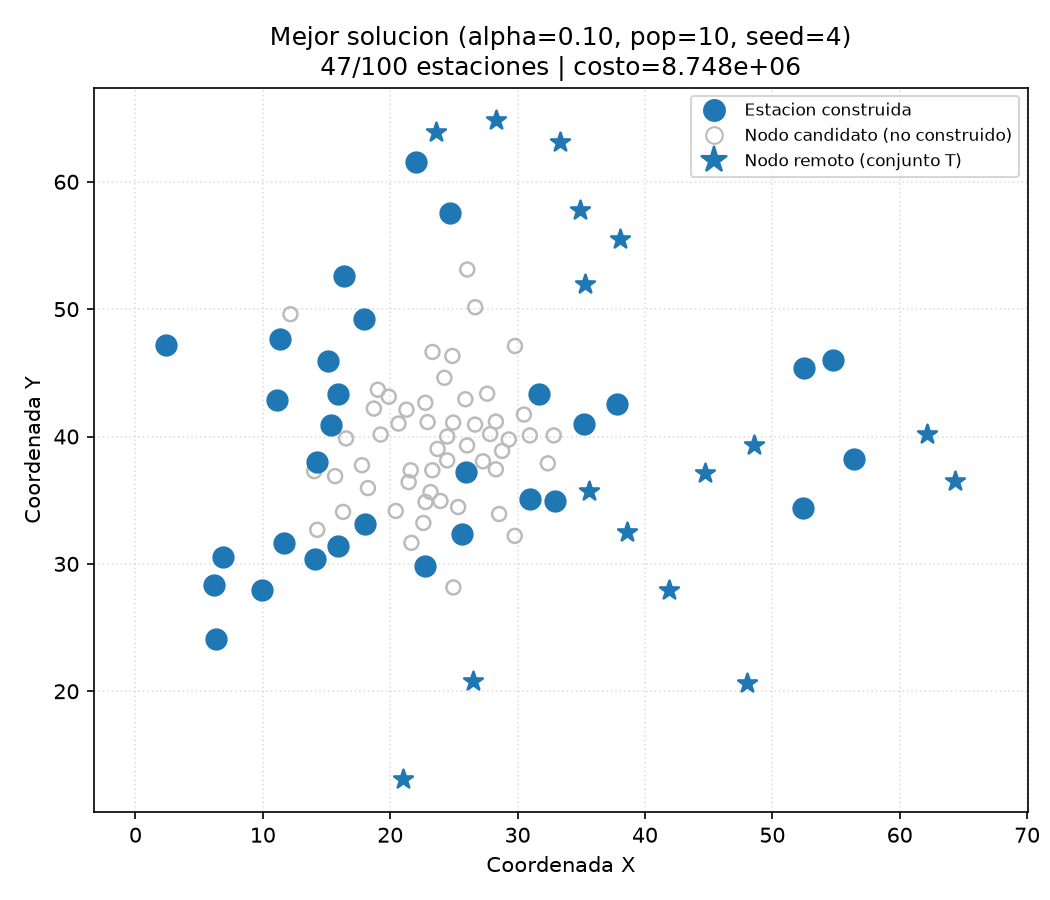
\includegraphics[width=0.55\textwidth]{images/mapa_solucion.png}
\caption{Solución representativa para $\alpha = 0.10$ (población $10$, semilla $4$): $47$ de $100$ estaciones construidas, costo $8.75 \times 10^6$.}
\label{fig:mapa}
\end{figure}

\textbf{Afinamiento del tamaño de la población.} El segundo experimento afina el único hiperparámetro
barrido, el tamaño de la población. La Figura~\ref{fig:costopop} presenta el costo relativo
(normalizado al mejor valor de cada $\alpha$) en función del tamaño de la población para los tres
valores de $\alpha$ factibles. En los tres casos el costo no mejora al aumentar la población; al
contrario, crece de forma monótona, y el efecto es más marcado cuanto más exigente es la instancia
(la mayor pendiente corresponde a $\alpha = 0.10$). Es decir, una población mayor no produce mejores
soluciones para este problema.

\begin{figure}[H]
\centering
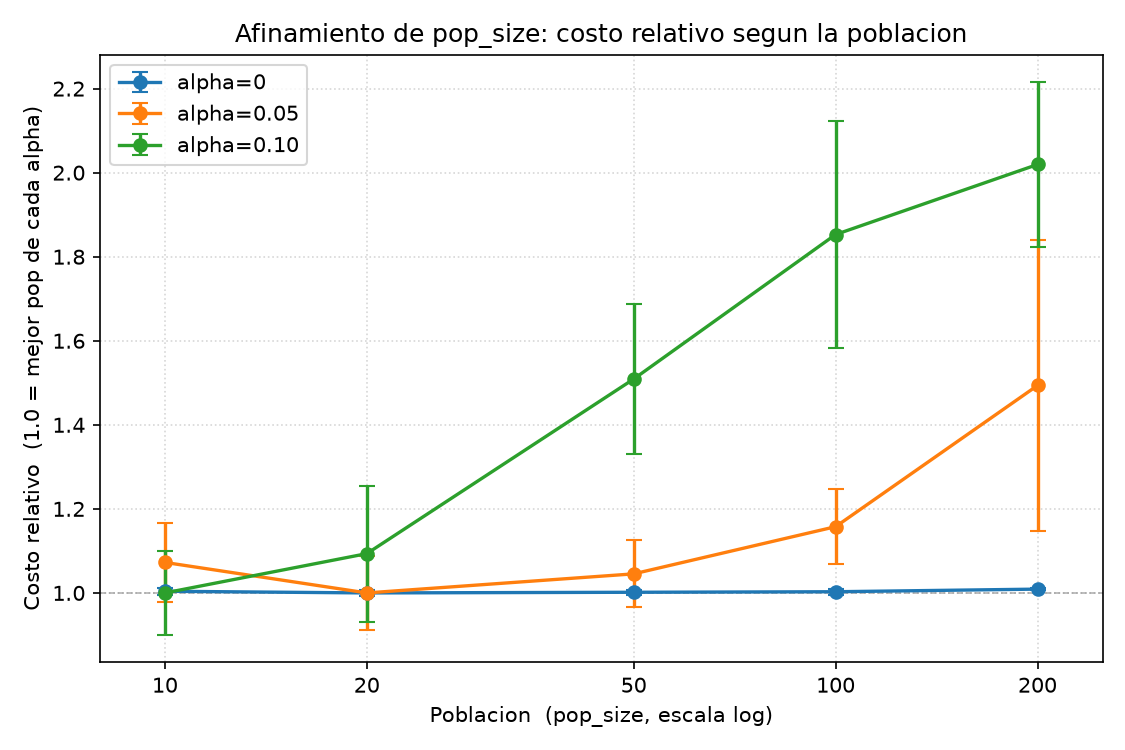
\includegraphics[width=0.6\textwidth]{images/costo_vs_pop.png}
\caption{Costo relativo (1.0 = mejor población de cada $\alpha$) según el tamaño de la población, para los tres valores de $\alpha$ factibles.}
\label{fig:costopop}
\end{figure}

Este resultado se refuerza al incorporar el esfuerzo computacional. La Figura~\ref{fig:costoesfuerzo}
superpone, para $\alpha = 0.10$, el costo de la solución y el esfuerzo (evaluaciones de la función de
aptitud) frente al tamaño de la población, y el Cuadro~\ref{tab:pop} entrega las cifras. Ambas
magnitudes crecen con la población, y el tamaño más pequeño, $N = 10$, minimiza las dos a la vez. En
términos concretos, pasar de $N = 10$ a $N = 200$ no solo no mejora el costo, sino que lo empeora (de
$9.64 \times 10^6$ a $1.95 \times 10^7$, un factor de $2.0$), y multiplica el esfuerzo por un factor
de $16.3$ (de unas $8\,200$ a $134\,000$ evaluaciones). Como además todas las configuraciones
alcanzan la factibilidad ($10/10$ en cada caso), la confiabilidad no es el factor que las distingue:
lo son el costo y el esfuerzo.

\begin{figure}[H]
\centering
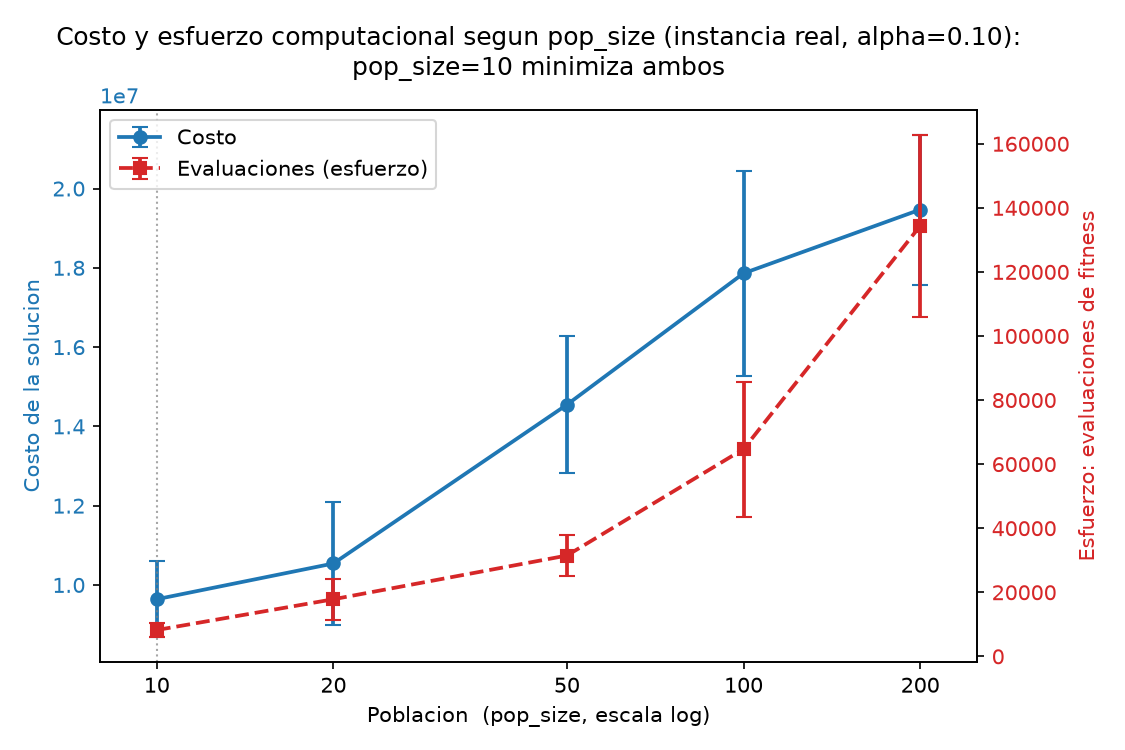
\includegraphics[width=0.6\textwidth]{images/costo_y_esfuerzo_vs_pop.png}
\caption{Costo de la solución y esfuerzo (evaluaciones) según el tamaño de la población, para $\alpha = 0.10$. El tamaño $N = 10$ minimiza ambos.}
\label{fig:costoesfuerzo}
\end{figure}

\begin{table}[h]
\centering
\caption{Costo, esfuerzo y factibilidad según el tamaño de la población, para $\alpha = 0.10$ (promedios sobre $10$ corridas factibles)}
\label{tab:pop}
\begin{tabular}{cccc}
\hline
Población $N$ & Costo medio ($\times 10^6$) & Evaluaciones medias & Factibilidad \\
\hline
$10$  & $9.64 \pm 0.91$  & $8\,220$   & $10/10$ \\
$20$  & $10.54 \pm 1.48$ & $17\,830$  & $10/10$ \\
$50$  & $14.55 \pm 1.63$ & $31\,475$  & $10/10$ \\
$100$ & $17.86 \pm 2.46$ & $64\,710$  & $10/10$ \\
$200$ & $19.47 \pm 1.79$ & $134\,380$ & $10/10$ \\
\hline
\end{tabular}
\end{table}

La conclusión del experimento es que, en este problema, la palanca del rendimiento no es el tamaño de
la población sino el esfuerzo invertido. Una población pequeña converge en un número de generaciones
similar (entre unas $600$ y $900$), pero a un costo por generación mucho menor, de modo que alcanza
mejores soluciones gastando una fracción del cómputo; una población grande, combinada con la
selección por ruleta, probablemente diluye la presión selectiva y consume el presupuesto sin una
mejora proporcional. Medir el esfuerzo en evaluaciones, y no en tiempo de reloj, fue lo que permitió
hacer visible este efecto.

\section{Conclusiones}

Este trabajo abordó el Problema de Ubicación de Estaciones de Carga para Vehículos Eléctricos
(EVCSPP) mediante un algoritmo genético, fiel a la formulación de Ou et al.
\cite{1_Solving_optimal_evcsp_problem_QUANTUM}. Sobre instancias reales de $100$ ubicaciones se
ejecutó un barrido de $250$ corridas que combinó el parámetro del problema $\alpha$ con el tamaño
de la población, empleando distintas semillas como réplicas. De los resultados se desprenden dos
conclusiones principales.

La primera concierne al papel del coeficiente $\alpha$. Su aumento lleva al modelo a seleccionar
redes progresivamente más dispersas y realistas, y reduce el número de estaciones construidas desde
prácticamente la totalidad de las candidatas con $\alpha = 0$ hasta cerca de la mitad con
$\alpha = 0.10$, con la consiguiente baja del costo. Sin embargo, este endurecimiento tiene un
límite estructural: a partir de $\alpha = 0.15$ las instancias se vuelven infactibles por
construcción, pues ninguna asignación de estaciones alcanza a cubrir la demanda. Esta frontera no es
una debilidad del algoritmo, sino una propiedad del problema, y conviene tenerla presente al definir
las instancias de prueba.

La segunda conclusión, y el hallazgo central del trabajo, es que en este problema el tamaño de la
población no es la palanca del rendimiento: lo es el esfuerzo computacional. Una población pequeña
($N = 10$) alcanzó soluciones de menor costo que una población veinte veces mayor ($N = 200$),
gastando alrededor de dieciséis veces menos evaluaciones de la función de aptitud. Medir el esfuerzo
en evaluaciones, y no en tiempo de reloj, fue determinante para evidenciar este efecto, que habría
quedado oculto al comparar únicamente el costo final. El resultado advierte contra la suposición
intuitiva de que una población mayor siempre mejora la búsqueda.

Como trabajo futuro se identifican dos líneas concretas. La primera es extender el ajuste a otros
parámetros del algoritmo que en esta iteración se mantuvieron fijos, como la tasa de cruzamiento o
la paciencia del criterio de término. La segunda es afinar la grilla de $\alpha$ entre $0.10$ y
$0.15$ (valores $0.11$, $0.12$, $0.13$ y $0.14$) para ubicar con precisión el punto exacto en que el
problema deja de tener solución, caracterizando así la frontera de factibilidad. Ambas direcciones
permitirían robustecer las conclusiones y profundizar en la relación entre la dificultad de la
instancia y el comportamiento del algoritmo.



\newpage

\section{Uso LLMs}

\begin{enumerate}
    \item Herramienta: Gemini 3.1 flash (Versión promocional estudiantes)
    \item Uso: Revisión de redacción, Resumen de fuentes, Depurar errores de latex.
    \item Prompt principal: Consultas información específica en fuentes: "De acuerdo a este \{abstract\} y a esta \{conclusión\} del recurso \{recurso\} se habla de \{tema\}?"
    \item Intervención: Si la IA me confirmaba o me negaba preguntas que tenía sobre una fuente, iba de nuevo a revisar la parte del texto con la que estaba (o no estaba) siendo coherente con mi idea.
    \item Apoyo en código: utilicé IA generativa como apoyo en el código de generación de los barridos experimentales, dado que existían optimizaciones posibles en esa rutina que yo no conocía, como la ejecución en paralelo de las corridas y la escritura incremental de los resultados a disco. Mi intervención consistió en auditar yo mismo el código, leyendo lo que proponía la IA y contrastándolo con otros casos de uso de ese tipo de optimizaciones antes de incorporarlo.
\end{enumerate}

\bibliographystyle{plain}
\bibliography{Referencias}

\end{document} 
